\subsection{System Model}\label{sec:model}

\begin{figure}[tb]
    \centering
    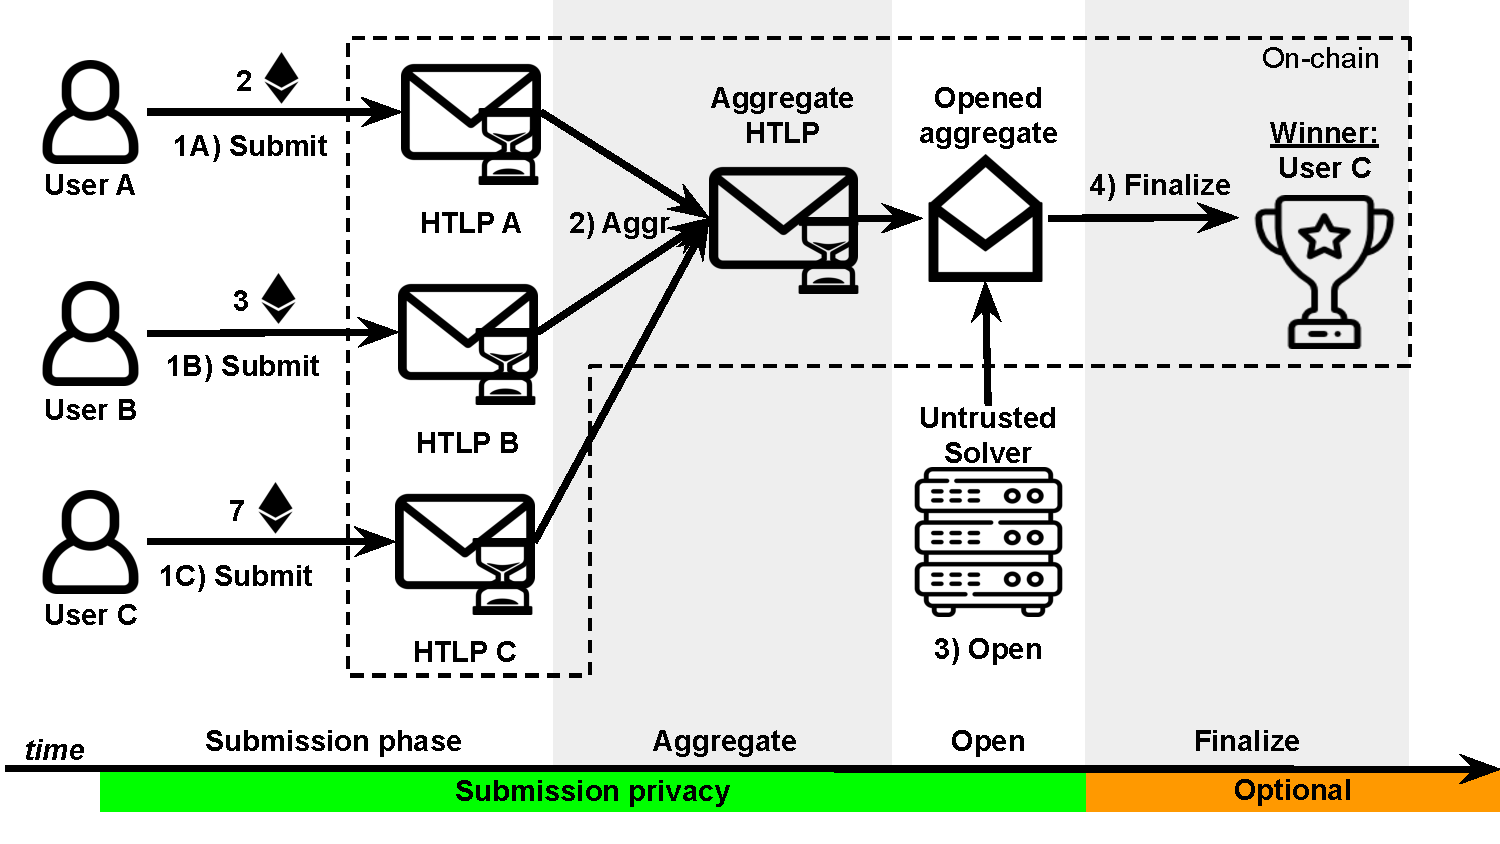
\includegraphics[width=0.95\textwidth]{cicada/figs/cicada-explainer.pdf}
    \caption{The system model of Cicada. \emph{(1) Submission phase:} users generate their bids/ballots as HTLPs and post them to a public bulletin board, e.g., a blockchain. \emph{(2) Aggregation:} an on-chain contract homomorphically combines submissions into an aggregate puzzle as they are submitted. \emph{(3) Opening:} after all submissions have been aggregated, an off-chain entity solves the aggregate HTLP using $\Ttime$ sequential steps and submits the solution to the contract. \emph{(4) Finalize:} The smart contract may do some final computation over the solution to compute the result and announces the winner. Submission privacy is ensured only until the start of the $\mathsf{Open}$ phase. 
    In \Cref{sec:everlasting_ballot_privacy}, we show how voters can pool their submissions to achieve everlasting ballot privacy.
    }
    \label{fig:cicada-explainer}
\end{figure}


Our system design is illustrated in \Cref{fig:cicada-explainer}. We envision three types of participants:
% \ifctb
% \emph{users}, who submit bids or ballots; an \emph{on-chain coordinator}, typically implemented as a smart contract, who collects submissions (bids or ballots) and transparently calculates the winner(s); and an \emph{off-chain solver}, who unlocks the final HTLP(s) off-chain and submits the solution(s) to the coordinator along with a proof of correctness.
% \else
\begin{description}
    \item[Users.] We simply refer to voters or bidders as \emph{users}. Users submit bids or ballots, which we generically call \emph{submissions}. We assume some external process to establish the set of authorized users (which may be open to all).  Once users place their submissions, no further action is required of them. 
    \item[On-chain coordinator.] We refer to the tallier/auctioneer as the \emph{coordinator}, typically implemented as a smart contract that collects submissions. The coordinator transparently calculates the winner(s). In the case of an auction, they might also transfer (digital) assets to the winner(s). In an election, they might grant special privileges to the winner.%'s public key.
    \item[Off-chain solver.] Since our protocols apply HTLPs, we assume an untrusted \emph{solver} who unlocks the final HTLP(s) off-chain and submits the solution(s) to the coordinator with proofs of correct opening attached. This could, in principle, be any party, although, in practice, it will likely be one of the parties participating in (or administering) the vote/auction, or a paid marketplace~\cite{EPRINT:Abadi23,CCS:TGBKS21}.
\end{description}

An adversary may attempt to read ballots/bids before the submission phase is complete. This is prevented by the security properties of (H)TLPs (\Cref{sec:background_tlp}) assuming the delay $\Ttime$ is longer than the submission phase.